% Define document class and reference
\documentclass{article}
\usepackage[left=2cm, right=2cm, bottom=2cm, top=2cm]{geometry}
\usepackage{graphicx} % Required for inserting images
\usepackage{siunitx}
\usepackage{amsmath}
\usepackage{placeins}
\usepackage{xcolor}
\usepackage{wrapfig}
\usepackage{amssymb}
\usepackage{tabularx}
\usepackage{bm}
\usepackage[table]{xcolor}
\usepackage{subcaption}
\usepackage[hidelinks]{hyperref}
\usepackage{cleveref}

% Figure caption setup
\captionsetup{font=footnotesize,labelfont=bf}

% Matrix and vector notation
\newcommand\matr[1]{\ensuremath{\boldsymbol{\mathbf{#1}}}}
\newcommand\vect[1]{\ensuremath{\bm{#1}}}

% Define title
\renewcommand{\refname}{}

% ADD THE FOLLOWING COUPLE LINES INTO YOUR PREAMBLE
\let\OLDthebibliography\thebibliography
\renewcommand\thebibliography[1]{
	\OLDthebibliography{#1}
	\setlength{\parskip}{0pt}
	\setlength{\itemsep}{3pt plus 0.3ex}
}

\def\corr#1{{\color{black}{#1}}} % final corrections


\begin{document}
	
\begin{figure}[h]
	\raggedleft
	
\includegraphics[width=3cm]{figures/uni_bern.png}
\end{figure}

%\vspace{-0.5cm}
%\noindent \large \textbf{\color{red} DRAFT VERSION 4}
\normalsize

\subsection*{Research Project for Graduate School of Biomedical and Precision Engineering}
\renewcommand{\arraystretch}{1.3}
\begin{table}[h!]
	\centering
	\begin{tabularx}{\textwidth}{|l|X|}
		\hline
		\textbf{Name} & Daniel Zahnd \\
		\hline
		\textbf{Project title} & The METAS joule-watt balance: A combined realization \\
		\hline
	\end{tabularx}
\end{table}
\renewcommand{\arraystretch}{1.0}

\subsubsection*{Background} % Max. 1 page
Originally, the so-called Kibble balance – also known as the watt balance – was invented by \cite{Kibble1976} as a device to measure the gyromagnetic ratio of the proton, which subsequently led to the realization of the SI unit Ampere. With the discovery of the Josephson and quantum Hall effects, the Kibble balance became a tool to measure 
\begin{wrapfigure}{r}{0.35\textwidth}
	\centering
	\begin{subfigure}{0.34\textwidth}
		\centering
		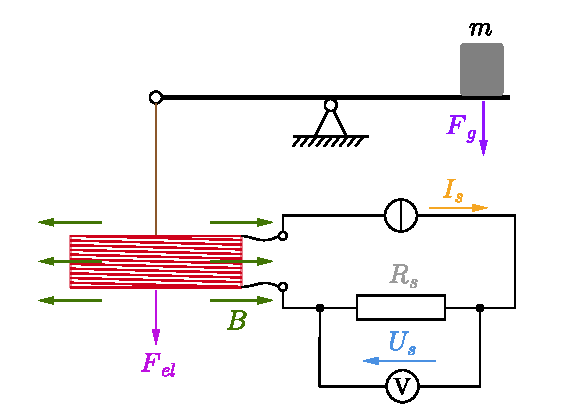
\includegraphics[width=\textwidth]{figures/balancestatic.pdf}
		\caption{Static mode of the Kibble balance.}
		\label{fig:balancestatic}
	\end{subfigure}
	\\
	\begin{subfigure}{0.34\textwidth}
		\centering
		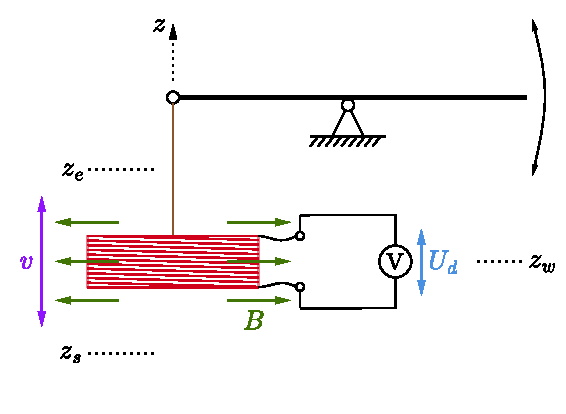
\includegraphics[width=\textwidth]{figures/balancedynamic.pdf}
		\caption{Dynamic mode of the Kibble balance.}
		\label{fig:balancedynamic}
	\end{subfigure}
	\caption{Visualization of the working principle of a Kibble balance.}
	\label{fig:kibblebalanceprinciple}
\end{wrapfigure}
the Planck constant $h$ with exceptional accuracy. Since the 2019 revision of the SI system, the Planck constant $h$ has a fixed value, hence the Kibble balance now can be used to realize the kilogram unit.

The fundamental principle of the Kibble balance is fairly simple and relies on fundamental principles from classical mechanics, electrodynamics and quantum physics. Essentially, the Kibble balance establishes a virtual comparison of mechanical and electrical power; therefore the balance is also known as a watt balance. As shown in \cref{fig:kibblebalanceprinciple}, it can be pictured as beam balance, where on one end a mass $m$ is placed and at the other end a circular coil in a radial magnetic field is suspended. The balance is then operated in two modes: The static and dynamic mode. In the static mode, a weight $m$ is placed on the one end of the beam balance and a variable current $I_s$ flowing through the coil is used to balance the gravitational force $\vect{F}_g = m \vect{g}$ by the generated force \begin{equation}\vect{F}_{el} = I_s\oint \vect{B} \times  \mathrm{d}\vect{l},\end{equation} where $\vect{B}$ is the magnetic field and $\mathrm{d}\vect{l}$ is a line element of the coil. The current is measured by using a resistor $R_s$ and a digital voltmeter measuring the voltage drop $U_s$ over it. In the dynamic phase however, the weight is removed from the beam balance and instead the beam is moved up and down at a velocity $\vect{v}$. This movement of the coil induces a voltage \begin{equation}U_d = \oint (\vect{v}\times \vect{B})\cdot \mathrm{d}\vect{l} = \oint (\vect{B}\times \mathrm{d}\vect{l})\cdot \vect{v}\end{equation} in the coil measurable directly by the digital voltmeter. If it can be ensured that the geometrical factor $\oint \vect{B} \times  \mathrm{d}\vect{l}$ is identical in both the static and dynamic phases, one obtains the equation \begin{equation}\label{eq:kibblebalancefundamental}
	m\frac{g}{I_s} = \frac{U_d}{v}
\end{equation} relating the mass $m$ to the measured quantities $g=|\vect{g}|$, $v = |\vect{v}|$, $I_s$ and $U_d$, where $I_s$ and $U_d$ furthermore are directly related to the Planck constant $h$ by means of the Josephson and quantum Hall effects.

\subsubsection*{Hypotheses and aims}
Several national metrology institutes around the world are in possession of a Kibble balance or run an Avogadro project to realize the mass unit. As \cite{Stock_2023} indicate, the obtained realizations of the kilogram are however not yet in satisfactory agreement to allow for independent realizations of the mass unit. Until such agreement can be provided to a \corr{sufficient} degree, the kilogram realization is therefore given by a weighted\footnote{Realizations with a smaller measurement uncertainty have larger weight.} mean of realizations obtained by all contributing national metrology institutes (NMI's). Only through continuous improvement of the experiments in terms of accuracy, independent realizations will become possible.

The overarching goal of the proposed project is therefore to reduce the total measurement uncertainty of the METAS Kibble balance experiment. In order to reduce the total measurement uncertainty, a careful evaluation of each contributing source is necessary, especially of the most significant ones. The current total measurement uncertainty is reported by \cite{Eichenberger_2022} to be $4.3 \cdot 10^{-8}$ in relative terms. The proposed project aims to reduce this relative uncertainty to below $3.0 \cdot 10^{-8}$.

Hypotheses 1 and 2 aim at reducing these most significant measurement uncertainty contributions\corr{, which is a required precondition for the development of the joule balance mode constituting hypothesis 3.} As an aside, hypothesis 4 aims at leveraging machine learning techniques to simplify and accelerate measurements using the Kibble balance experiment.

\paragraph*{\normalfont \textsc{Hypothesis and aim 1:}}
\begin{wrapfigure}{r}{0.27\textwidth}
	\centering
	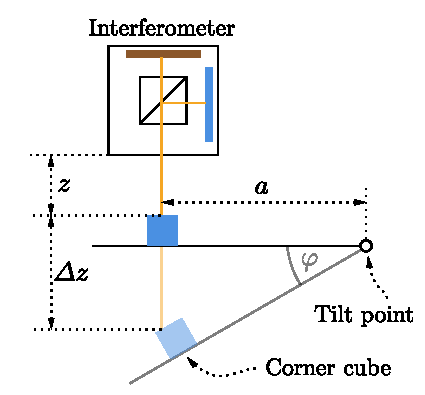
\includegraphics[width=0.27\textwidth]{figures/abbeerror.pdf}
	\caption{Visualization of a so-called Abbe offset error $\Delta z$.}
	\label{fig:abbeerror}
\end{wrapfigure}
The main contribution to the uncertainty budget of the current METAS Kibble balance setup is due to reproducibility, which is strongly dependent upon the noise present in the $U_d/v$ profile\footnote{The values of $U_d$ and $v$ are measured along the vertical axis $z$; one therefore obtains a profile $U_d/v$ with respect to $z$. See \cref{fig:U_d_over_v_profile} and \cref{fig:balancedynamic} for visualizations.}. 
The Abbe offset error, illustrated in \cref{fig:abbeerror}, is a significant source of noise in this profile. It occurs due to a tilt of the moving mirror in the interferometer system, leading to an error $\Delta z = a \varphi$ for small angles $\varphi \ll 1$ affecting distance measurement $z$. In the Kibble balance experiment, tilting of the coil supporting the mirrors during the dynamic phase introduces Abbe offset errors to distance measurements, affecting the calculated velocity $v$ but not the induced voltage $U_d$. This introduces noise in the ratio $U_d/v$. Mitigating these errors is crucial to minimizing noise in the $U_d/v$ profile. As a solution to mitigate these errors, the so-called 3-interferometer technique has been introduced by \cite{5544638} and successfully implemented in Kibble balance experiments worldwide, such as the NIST Kibble balance \cite{Haddad_2017} and the BIPM watt balance \cite{Fang_2020}.

The candidate hypothesizes therefore, that an implementation of the 3-interferometer technique will lead to an improvement in reproducibility of the Kibble balance experiment due to a reduction of noise in the $U_d/v$ profile.

\paragraph*{\normalfont \textsc{Hypothesis and aim 2:}}
\begin{wrapfigure}{r}{0.27\textwidth}
	\centering
	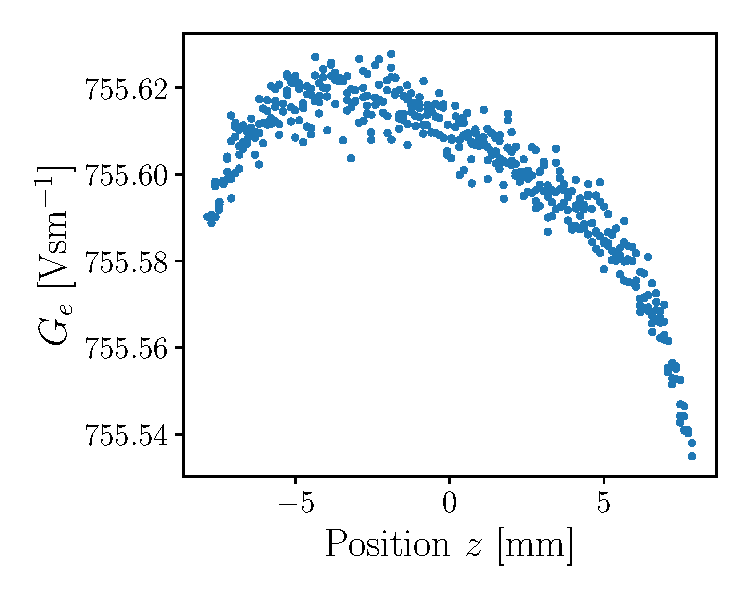
\includegraphics[width=0.27\textwidth]{figures/Ge_example.pdf}
	\caption{Example datapoints obtained for the $G_e = U_d/v$ profile.}
	\label{fig:U_d_over_v_profile}
\end{wrapfigure}
Curve fitting for $U_d/v$ measurements during the dynamic phase contributes significantly to the uncertainty budget, as \cite{Eichenberger_2022} write. Currently, the polynomial order is selected to avoid over- or underfitting, however lacking a physical model to justify a specific order.
This makes it necessary to perform different orders of fits and investigate the influence on the resulting calculated mass $m$; the spread of the obtained mass data $m$ then serves as the uncertainty contribution associated to choosing the appropriate fit order. The choice of fit order furthermore becomes more arbitrary with higher noise levels in the $G_e \doteq U_d/v$ profile. To reduce the uncertainty contribution due to curve fitting, finding the optimal polynomial order backed by physical reasoning is crucial. In the ideal case, the $G_m \doteq g/I_s$ profile exactly mirrors the $G_e$ profile and is much less prone to noise, because the measurements take place in a static, rather than dynamic setup as it is the case for the $G_e$ profile. The $G_m$ profile can be obtained through weightings at locations $z \in [z_s, z_e]$ of the dynamic range aswell as by finite element simulations (FEM) of the magnetic field and coil interaction during the dynamic phase.

The candidate hypothesizes, that obtaining a $G_m$ profile across the dynamic range will help to choose the most appropriate polynomial fit order and thereby lead to a reduction of the associated uncertainty contribution.

\paragraph*{\normalfont \textsc{Hypothesis and aim 3:}}
When two independent measurement methods are employed for the same quantity, the uncertainty of their mean value is smaller than that of each individual method, even if they are correlated. In this research project, utilizing the METAS Kibble balance as a joule balance offers an alternative measurement approach alongside the conventional Kibble balance mode. The joule balance mode compares mechanical to electrical work - rather than power as in the watt balance mode - and is governed by the equation \begin{equation}\label{eq:joulebalance}
	m\int_{z_s}^{z_e}\frac{g(z)}{I(z)}\,\mathrm{d}z = \int_{t(z_s)}^{t(z_e)} U(t)\,\mathrm{d}t,
\end{equation} involving measurements of gravitational acceleration $g(z)$, weighting currents $I(z)$, and induced voltages $U(t)$. The feasibility of a joule balance mode has been shown by \cite{Xu_2016}.

The candidate hypothesizes that modifying the METAS Kibble balance such that one can obtain a Kibble balance and joule balance measurement for the same mass could further decrease measurement uncertainty, since two measurement methods for the same mass would be provided.

\paragraph*{\normalfont \textsc{Hypothesis and aim 4:}}
\begin{wrapfigure}{r}{0.16\textwidth}
	\centering
	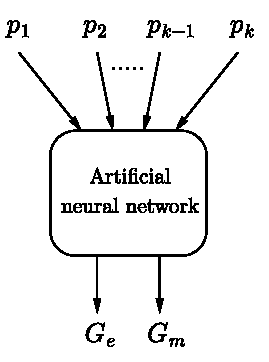
\includegraphics[width=0.15\textwidth]{figures/nn.pdf}
	\caption{Proposed architecture of the neural network; $\vect{p}$ are the alignment parameters and $\vect{q}$ are the geometrical factors associated to the alignment parameters.}
	\label{fig:nn}
\end{wrapfigure}
Operating the METAS Kibble balance in the conventional mode requires an alignment procedure to be carried out prior to mass determination. 
By means of systematically introducing variations to the alignment parameters $\vect{p} \doteq \{p_1,\dots,p_n\}$ of the setup, the effect these variations have on the calculated values of the geometrical factors $\vect{q} \doteq \{G_e, G_m\}$ can be studied. Thus, if one has a set of parameter values $\matr{p} = \{\vect{p}_1,\dots,\vect{p}_k\}$ with a corresponding set of calculated geometrical factors $\matr{q} = \{\vect{q}_1,\dots,\vect{q}_k\}$, a training dataset for an artificial neural network can be obtained. Using such a dataset as ground truth, a neural network can be trained to learn correlations between the alignment parameters and the resulting geometrical factors, as indicated by the proposed architecture \cref{fig:nn}.
This also means, that the neural network will learn correlations between possible misalignment of the experimental setup and resulting deviations of the geometrical factors from their respective optimal values. If the optimal alignment parameters and the actual alignment parameters of a particular experimental setup are known/measured, the trained neural network then allows to calculate the correction for the geometrical factors due to a non-optimal alignment of the experiment. 

The candidate hypothesizes, that training a machine learning algorithm (artificial neural network) to learn correlations between alignment parameters and resulting geometrical factors could contribute to making measurements with the METAS Kibble balance faster, more convenient and therefore more cost-efficient.

\subsubsection*{Methods and research plan}
In order to address the hypotheses developed above, the candidate proposes the following research plan consisting of seven key milestones:

\paragraph*{\normalfont \textsc{Milestone 1:}}
Achieve familiarity with the METAS Kibble balance by understanding its physical  and engineering principles. Conduct a complete measurement campaign involving adjustment, alignment, measurement, data processing and interpretation of the results.

\paragraph*{\normalfont \textsc{Milestone 2:}}
Metrologically characterize the commercial PicoScale interferometer system and implement the 3-interferometer technique for the METAS Kibble balance. Success in this endeavor will be a major contribution to a possible future implementation of a METAS table top realization of a Kibble or joule balance. Results are planned to be published.

\paragraph*{\normalfont \textsc{Milestone 3:}}
Complete required lectures and possibly attend a summer school on metrology or a related topic. Conduct gravimetric measurements in the Swiss alps. Results are planned to be published.

\paragraph*{\normalfont \textsc{Milestone 4:}}
Get familiar with software such as COMSOL for finite element simulations. Establish a $G_m = g/I_s$ profile through finite element simulation of coil interactions with the magnetic field and validate it with actual measurements of the profile. Determine suitable polynomial order for fitting the $G_e = U_d/v$ profile.

\paragraph*{\normalfont \textsc{Milestone 5:}}
Gather data of alignment parameters $\vect{p}$ and associated geometrical factors $\vect{q}$. Generate a training dataset using the acquired measurement data, build and train an appropriate AI model to learn correlations between alignment parameters and associated geometrical factors. Put the obtained AI model to the test and evaluate its performance, aswell as its usefulness and reliability.

\paragraph*{\normalfont \textsc{Milestone 6:}}
Develop the METAS joule balance mode to provide an alternative method to realize the mass unit. Create an associated uncertainty budget through thorough evaluation of all known uncertainty contributions. Compare results from both modes. Results are planned to be published.

\paragraph*{\normalfont \textsc{Milestone 7:}}
Compile project findings into the PhD thesis, including detailed treatment of relevant physics and engineering principles behind Kibble and joule balance modes. Conclusively address the proposed hypotheses.

%\paragraph*{\textit{Milestone 1:}}
%The first milestone will be to familiarize with the METAS Kibble balance as it is. This includes a detailed understanding of each physical principle employed by the balance aswell as of conducting a complete measurement campaign consisting of adjusting/aligning the components of the experiment, performing measurements and processing the obtained data.
%
%\paragraph*{\textit{Milestone 2:}}
%As a second milestone, the successful implementation of the 3-interferometer technique with the METAS Kibble balance is aspired. This will involve a metrological characterization of the used commercial PicoScale interferometer system. If it can be shown that a commercial interferometer system such as the PicoScale manufactured by SmarAct can be used for this technique, it will be considered as a major contribution to a possible future implementation of a METAS table top Kibble or joule balance. The obtained findings of this milestone are planned to culminate in a publication.
%
%\paragraph*{\textit{Milestone 3:}}
%The third milestone consists of successful completion of the required lectures and possibly a summer school on metrology. Furthermore, the milestone encompasses gravimetric measurements along a calibration line in the Swiss alps to get familiar with gravimetric measurements. This is also planned to result in a publication.
%
%\paragraph*{\textit{Milestone 4:}}
%The fourth milestone then is to establish a $G_m = g/I_s$ profile by a finite element simulation of coil interactions with the magnetic field and to validate this profile by doing actual measurements with the Kibble balance. This will help to choose the appropriate polynomial order for fitting the $G_e = U_d/v$ profile.
%
%\paragraph*{\textit{Milestone 5:}}
%As a fifth and culminating milestone, the development of the METAS joule balance mode is to be achieved. This will allow to determine the same mass $m$ using the watt and joule balance modes. Establishing an uncertainty budget for the joule balance mode will require a careful (re)-evaluation of all known uncertainty contributions. A comparison of obtained results for both modes is aspired to lead to another publication.
%
%\paragraph*{\textit{Milestone 6:}}
%The final milestone will be to gather, arrange and summarize the findings obtained throughout the project to write the PhD-thesis. Alongside a careful treatment of these findings, the PhD-thesis will also include a detailed treatment of all relevant physics and engineering principles leveraged by the Kibble and joule balance modes. The thesis should finally give conclusive answers to the above proposed hypotheses. 

\subsubsection*{Possible pitfalls and their solutions}
\paragraph*{\normalfont \textsc{Challenges concerning hypothesis 1:}} The realization of the 3-interferometer technique will require a metrological characterization of the used PicoScale interferometer system. Crucial for this interferometer system is the stability of the laser wavelength; this ensures, that the measured distances are stable over time. 

If it should however turn out that the wavelength of the interferometer system is not as stable as expected over long-term periods, the calibration intervals could be reduced in combination with a corresponding correction of measurements obtained in between calibrations.

\paragraph*{\normalfont \textsc{Challenges concerning hypothesis 2:}} In order to substantiate a choice of a certain order of polynomial to fit the $U_d/v$ profile datapoints, a $g/I_s$ profile needs to be measured. Due to the mechanical setup of the current METAS Kibble balance however, such a profile can at present stage only be captured over a vertical distance of $\SI{5}{\milli\meter}$. It is to be expected, that such a profile covers an insufficient distance along the vertical axis $z$ to substantiate the polynomial order choice of the fit for the $U_d/v$ datapoints. 

This problem could however be resolved by performing mechanical adjustments to the Kibble balance, such that one can perform weightings over a larger range up to $\SI{16}{\milli\meter}$.

\paragraph*{\normalfont \textsc{Challenges concerning hypothesis 3:}} The development of the joule balance mode for the existing METAS Kibble balance will require multiple weightings along the vertical axis $z$. Weightings are performed by introducing a current $I_s$ to the coil as indicated by \cref{fig:balancestatic}. These currents lead to heating of the permanent magnets producing the magnetic field $\vect{B}$ due to their proximity to the coil. Since the magnetic field is temperature dependent, strict temperature control for the magnets is required. In the watt balance mode, the temperature fluctuations due to currents flowing in the coil are compensated naturally, because after each static phase, a dynamic phase follows, where the temperature between the static and dynamic phases is sufficiently stable. The idea for the joule balane mode however is, that many static measurements are performed after one another, before a dynamic measurement is carried out. Hence, it is unclear whether the temperature of the magnetic system will be sufficiently stable over the whole period of static and dynamic measurements.

The problem of heating effects not naturally being compensated in the joule balance mode could be addressed by either correcting the measurements using the known temperature coefficient of the magnetic field $\vect{B}$, or by operating the joule balance mode such that it essentially just consists of many watt balance measurements along the vertical direction $z$.

\paragraph*{\normalfont \textsc{Challenges concerning hypothesis 4:}} With respect to hypothesis 4 it is yet unclear, if a sufficiently dense dataset for training a machine learning algorithm will be acquired during the PhD project. The performance of the trained algorithm is expected to scale with the variation and hence the amount of training data.

However, a possible solution to an insufficient training dataset would be to densify it by creating a digital twin model of the Kibble balance and to simulate data with it.


%A challenge that might need addressing is outgassing on behalf of parts of the experimental apparatus due to performing measurements in vacuum. It has been observed in the past, that outgassing might lead to condensation of material on the test mass and thus to a gain in mass during the experiment. A possible solution to this problem might be a stable pressure control during the measurements performed under vacuum.

\subsubsection*{Collaborators}
The PhD project takes place in collaboration of the Swiss Federal Institute of Metrology (METAS) with the Graduate School for Biomedical and Precision Engineering at the University of Bern. The project is funded by METAS by means of employment of the candidate. There might be further collaborations with the industrial partners SmarAct and Mettler-Toledo, which are the manufacturers of some parts used in the Kibble balance experiment as it is of today.

\subsubsection*{Significance}
The research plans presented above aim for an increasingly accurate and stable national and international realization of the kilogram and herewith indirectly contribute to the well-being of economies and societies, because standardization of units is crucial to industry and commercial endeavors.

\FloatBarrier
\subsubsection*{Timetable}
\vspace{-0.2cm}

\begin{table}[h]
	\footnotesize
	\centering
	\begin{tabularx}{\textwidth}{|X|c|c|c|c|c|c|c|}
		\hline
		& FS24 & HS24 & FS25 & HS25 & FS26 & HS26 & FS27 \\
		\hline
		- Familiarization with the existing METAS Kibble balance \newline
		- Underst. the basic physical principles employed by the Kibble balance\newline
		- Conduct complete measurement campaign involving all key steps
		& \multicolumn{1}{>{\columncolor{lightgray}}c|}{} & & & & & &\\ 
		\hline
		- Attending lectures \newline
		- Implementation of 3-interferometer technique
		& 
		& \multicolumn{1}{>{\columncolor{lightgray}}c|}{} &  &  &  & & \\
		\hline
		- $1^{\text{st}}$ \textbf{paper} on 3-interferometer technique\newline
		- Attending lectures\newline
		- Gravimetric calibration line
		& & & \multicolumn{1}{>{\columncolor{lightgray}}c|}{} & & & & \\
		\hline
		- $2^{\text{nd}}$ \textbf{paper} on gravimeter measurements \newline
		- Research towards substantiating well-chosen polynomial fit order \newline
		- Reevaluation of the uncertainty budget for the Kibble balance mode\newline
		- Build and train AI model to predict corrections for misalignm. of setup
		&
		&
		&  & \multicolumn{1}{>{\columncolor{lightgray}}c|}{} &  & & \\
		\hline
		- Modification of the Kibble balance to operate it as a joule balance\newline
		- Establishing an uncertainty budget for the joule balance mode\newline
		- Comparison of Kibble balance vs. joule balance modes/results
		&
		&
		&
		&  & \multicolumn{1}{>{\columncolor{lightgray}}c|}{} &  & \\
		\hline
		- $3^{\text{rd}}$ \textbf{paper} on a comparison of Kibble balance vs. joule balance modes\newline
		- Writing the PhD thesis
		&
		&
		&
		&
		&  & \multicolumn{1}{>{\columncolor{lightgray}}c|}{} & \\
		\hline
		- Writing the PhD thesis and preparing the defense
		&
		&
		&
		&
		&
		&  & \multicolumn{1}{>{\columncolor{lightgray}}c|}{} \\
		\hline

	\end{tabularx}
\end{table} %\multicolumn{2}{>{\columncolor{lightgray}}c|}{}
\normalsize
\vspace{-0.5cm}
\FloatBarrier

\subsubsection*{References}
\vspace{-8.5mm}
\small
\bibliography{references}
\bibliographystyle{apalike}
\normalsize

\subsubsection*{Approval}
\noindent
I confirm to have discussed the research project with the student. Further, I confirm to have read the research proposal in its entirety and agree with this research project, timeline, and goals. 

\vspace{1.0cm}\noindent
Date and place: \hspace{6cm} Signature supervisor:


\end{document}